\problemname{Dartboard}

Jaap is playing darts at the local pub with a group of friends. His
darts throwing skills are not that great, so he just tries to aim at
the center of the dartboard. His mathematical skills are better
though, and he wonders what is his expected score for one dart.

After a while Jaap estimates that his darts hit the dartboard (or
often miss it) with a probability distribution that depends only on
the radius $r$ from the center of the board, and has the Gaussian form%
\footnote{This implies that the total probability is never larger than one.}
\[
  f(r) = \frac{1}{2\pi\sigma^2} e^{-\frac{r^2}{2\sigma^2}}.
\]
That is, the probability of hitting a small surface area
$\Delta x\!\cdot\!\Delta y$ at a distance $r$ from the center is given
by $f(r) \Delta x\!\cdot\!\Delta y$. Here $\sigma$ denotes the
standard deviation, and Jaap found out that this depends strongly on
how many beers he has had.

For those not familiar with the game of darts, a dartboard is depicted
below. The score for hitting each of the regions of the dartboard is
as follows:
\begin{itemize}\setlength{\itemsep}{0pt}
\item the inner \emph{bull's eye} is worth $50$ points;
\item the \emph{bull} annulus is $25$ points;
\item each pie has worth of the respective number $1$ up to $20$, but
\item the inner \emph{triple ring} has triple the worth of the pie, while
\item the outer \emph{double ring} has double the worth.
\end{itemize}
Finally, if the dart lands outside the double ring, the score is zero.
Note that the pies of all numbers have equal area.

\begin{figure}[h]
  \centering
  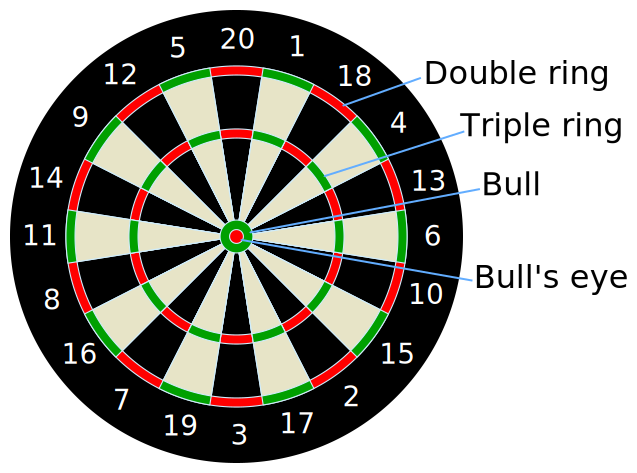
\includegraphics[width=6cm]{dartboard}
  \caption{A standard dartboard (from Wikimedia, CC BY-SA 3.0 licensed by Tijmen Stam).}
  \label{fig:dartboard}
\end{figure}

\section*{Input}

The first line contains 6 floating point
numbers of strictly increasing size: the radii of the
\emph{bull's~eye}, \emph{bull}, inner and outer \emph{triple ring},
and inner and outer \emph{double ring}, all in centimeters. The second
line contains the standard deviation $\sigma$ in centimeters as a
floating point number. All floating point numbers are in the range
$[10^{-3}, 100]$.

\section*{Output}

Print the expected score of one dart for Jaap as a floating point
number on a single line. The answer should be correct up to either a
relative or absolute error of $10^{-4}$.


%%% Local Variables: 
%%% mode: latex
%%% TeX-master: t
%%% TeX-PDF-mode: t
%%% End: 
